% !TEX program = xelatex
% Final Chinese paper. Layout follows the supplied PA-RCB-UOT reproduction package.
\documentclass[10pt,a4paper,fontset=windows]{ctexart}
\usepackage[margin=0.78in]{geometry}
\usepackage{amsmath,amssymb,amsthm,mathtools,bm}
\usepackage{booktabs,tabularx,array,multirow,longtable}
\usepackage{graphicx,float}
\usepackage{xcolor,hyperref,cleveref,enumitem,caption,microtype,url,xspace}
\usepackage{algorithm,algpseudocode}
\usepackage{tikz}
\usetikzlibrary{arrows.meta,positioning,fit}
\hypersetup{hypertexnames=false,colorlinks=true,linkcolor=black,citecolor=blue!55!black,urlcolor=blue!55!black,pdftitle={GC-HiWA：可拒绝的无监督结构化坐标恢复},pdfauthor={蔡文傑}}
\floatname{algorithm}{算法}
\setlength{\parindent}{2em}
\renewcommand{\arraystretch}{1.08}

\newcommand{\RR}{\mathbb{R}}
\newcommand{\OO}{\mathrm{O}}
\newcommand{\SO}{\mathrm{SO}}
\newcommand{\norm}[1]{\left\lVert #1\right\rVert}
\newcommand{\inner}[2]{\left\langle #1,#2\right\rangle}
\newcommand{\tr}{\operatorname{tr}}
\newcommand{\diag}{\operatorname{diag}}
\newcommand{\Proj}{\operatorname{Proj}}
\newcommand{\argmin}{\operatorname*{arg\,min}}
\newcommand{\argmax}{\operatorname*{arg\,max}}
\newcommand{\softmax}{\operatorname{softmax}}
\newcommand{\U}{\mathcal U}
% Allow TeX a small amount of additional flexibility in dense Chinese prose;
% this prevents isolated line overflow without changing the page geometry.
\setlength{\emergencystretch}{1.2em}
\newcolumntype{Y}{>{\raggedright\arraybackslash}X}
\newcolumntype{C}{>{\centering\arraybackslash}X}

\newtheorem{theorem}{定理}
\newtheorem{proposition}[theorem]{命题}
\newtheorem{lemma}[theorem]{引理}
\theoremstyle{definition}
\newtheorem{definition}[theorem]{定义}
\theoremstyle{remark}
\newtheorem{remark}[theorem]{注记}

\title{\textbf{GC-HiWA：可拒绝的无监督结构化坐标恢复}\\[0.45em]
\large 基于分层最优传输、ROCA 资格判定与受控三维姿态验证}
\author{蔡文傑\\厦门大学\\\href{mailto:19020232202343@stu.xmu.edu.cn}{19020232202343@stu.xmu.edu.cn}}
\date{}

\begin{document}
\maketitle

\begin{abstract}
无监督最优传输常被用于跨域对齐，但低传输代价或数值收敛本身不能证明两个域具有可迁移的共同结构。本文研究一个更窄且可证伪的问题：给定两个无配对、无目标标签的数据域，当它们共享群组几何，且坐标关系可由预先声明的结构化正交变换表示时，能否恢复该变换；当这一条件不成立时，能否以明确原因弃权。为此，本文提出 GC-HiWA（\emph{Group-Conditioned Hierarchical Wasserstein Alignment}）。方法以旋转等变的整体标量标准化和软群组为基础，在群组层与样本层分别求解熵正则最优传输，并通过局部旋转与全局结构化旋转的 ADMM 共识估计坐标映射。对于三维姿态，允许族被限制为 $I_J\otimes SO(3)$，从而保证全部关节共享同一个物理相机旋转。我们进一步提出 ROCA（\emph{Representative-Oriented Component-Aware} qualification），在 $O(d)$ 的正、负行列式候选分支之间执行保守的资格选择；ROCA 不将 OT 目标误解为语义正确性，在候选不唯一或不健康时返回弃权。

GC-HiWA 的输出由数学合同约束：局部 OT 边际、正交性、单旋转拟合比、协方差谱必要条件、可识别性间隔和多启动稳定性必须同时通过。在独立合成种子批次中，三个可恢复条件获得 $15/15$ 接受，五类预声明违例获得 $25/25$ 弃权；一个协方差谱完全相同、但不存在单一正交真值的非正交反例也被 $5/5$ 弃权。在 Panoptic Studio 的受控跨相机三维骨架实验中，拟合阶段不使用相机外参、同步帧或动作标签；结构化模型在三组相机配置的 11 次运行中均收敛，最大旋转误差为 $0.0308$，事后配对 Recall@1 均为 $1.0$。本文主张的是带失败诊断的无监督坐标恢复，而非任意跨域任务上的普适迁移提升。真实跨设备语义动作识别的冻结验证被明确保留为后续工作。
\end{abstract}

\noindent\textbf{关键词：}无监督坐标对齐；分层最优传输；三维姿态；正交 Procrustes；选择性弃权；适用性诊断

\begin{quote}\small
\textbf{本文的中心立场。} 对齐系统不应只输出一个数值矩阵；它还应说明该矩阵是否满足可部署的几何与数值条件。GC-HiWA 因而输出“结构化坐标变换”或“弃权及原因”，而不是在每个输入上强制生成映射。
\end{quote}

\section{引言}

\subsection{研究背景}
跨设备、跨相机或跨实验批次的数据往往描述同一物理对象，却使用不同坐标框架。三维骨架尤其典型：同一姿态在不同相机坐标系中的数值不同，直接将源相机训练的模型应用到目标相机通常会失效。若目标端缺少标定、样本配对和训练标签，问题就成为无监督坐标恢复。

最优传输（optimal transport, OT）为无配对分布比较提供了自然工具\cite{peyre2019computational,cuturi2013sinkhorn}。不过，OT 总能在给定代价下生成耦合；求解器收敛也只说明达到某一数值固定点。它们都不自动蕴含：一个单一的物理坐标变换存在、群组对应正确，或下游语义任务能够迁移。将数值拟合直接等同于语义迁移，是无监督对齐中最危险的解释跳跃。

分层 OT 方法表明：在具有稳定多模态或群组结构时，同时刻画群组间与群组内的对应可以提升对齐的可解释性\cite{lee2019hierarchical}。GC-HiWA 从这一思想出发，但把问题的重点从“如何始终输出一个对齐”改为“何时有资格输出一个对齐”。这导致方法、实验与论文主张均需要显式的适用性合同。

\subsection{问题与贡献}
本文的目标不是通用领域适配，而是如下受限问题：
\begin{quote}
在没有样本配对和目标标签时，若两个域共享群组几何并且只相差一个预声明的结构化正交坐标变换，则恢复该变换；若证据与此模型冲突，则拒绝输出。
\end{quote}

本文的主要贡献如下。
\begin{enumerate}
  \item \textbf{结构化坐标恢复合同。} 我们将允许变换族、数据几何、群组可比性与评价泄漏边界明确写出。对于 $J$ 个三维关节，使用 $I_J\otimes SO(3)$ 代替无物理意义的 $O(3J)$。
  \item \textbf{GC-HiWA 主干。} 我们给出由旋转等变标准化、全支持软群组、组条件局部 OT、组间熵正则 OT 与局部--全局旋转共识构成的可执行目标。
  \item \textbf{ROCA 与资格弃权。} 我们将 $O(d)$ 的行列式分支选择变为候选资格判定；候选冲突或证据不足时，系统保守弃权。
  \item \textbf{恢复边界证据。} 我们以独立种子验证可恢复条件、预声明失配、谱伪装非正交反例和受控真实相机几何，而不把失败数据集删除或包装为成功。
  \item \textbf{可追溯研究交付。} 代码、冻结 JSON、自动证据审计器、回归测试、论文源文件和限制说明均进入同一仓库。
\end{enumerate}

\section{相关工作与定位}

\subsection{最优传输与熵正则耦合}
经典 Kantorovich OT 在两个概率测度之间寻找满足边际约束的最低代价耦合。Sinkhorn 熵正则使这类问题具有高效且稳定的迭代求解形式\cite{cuturi2013sinkhorn,peyre2019computational}。本文使用熵正则并非因为它保证“真实配对”，而是因为它提供了明确边际与可检查的局部耦合。传输计划是几何证据的一部分，而不是标签的替代品。

\subsection{分层对齐与正交 Procrustes}
Lee 等提出的 HiWA 将聚类结构写成嵌套传输：外层 $P$ 匹配群组，内层 $Q_{ij}$ 解析群组内的样本质量，并通过局部 $R_{ij}$ 与全局 $R$ 的 ADMM 共识学习同一正交映射\cite{lee2019hierarchical}。因此，本文的双层 OT、Birkhoff 群组边际、局部--全局变量分裂和 Sinkhorn--ADMM 求解均有明确来源；后文重写这些公式，是为把原论文的硬簇记号变为可审计的软测度记号，而不是把已有理论误写成新推导。正交 Procrustes 则给出固定耦合时的闭式正交投影\cite{umeyama1991least}。GC-HiWA 在此基础上只增加两项受证据约束的限制：姿态任务使用物理结构化旋转族；估计结果必须通过适用性诊断才可进入下游。

\subsection{基于 HiWA 的软聚合扩展}
本文在 HiWA 的层级传输框架上直接引入软聚合：以可学习原型为中心，让每个样本以不同权重参与多个群组；由逐行归一的软隶属度构造组内经验测度，再以群组传输决定哪些局部几何证据参与全局共识。这样做不改变 HiWA 的群组--样本两层对齐骨架，却避免将样本硬性归入唯一群组。

本文只保留与无标签坐标恢复直接相关的部分：软原型、列归一化的局部质量、full-support 组内耦合、局部旋转和全局共识。项目中曾实现的组件条件样本代价是独立探索项，默认权重为零，且在当前神经--运动数据上未形成稳定双指标收益，故不计入 GC-HiWA 的冻结主干。

\subsection{选择性预测与本工作的弃权机制}
选择性预测研究通常通过置信度或显式拒绝头，在覆盖率与风险之间权衡\cite{geifman2019selectivenet}。GC-HiWA 的弃权不是分类置信度阈值：它针对的是\emph{结构化坐标模型是否存在并可识别}。因此诊断量来自 OT 边际、单旋转拟合、谱不变量、几何间隔和多启动一致性，而不是目标标签上的分类损失。

\subsection{与现有路线的区别}
\begin{table}[H]
\centering
\caption{方法定位比较。}
\label{tab:positioning}
\begin{tabularx}{0.96\linewidth}{lYYY}
\toprule
方法类别 & 已解决的问题 & 关键假设 & GC-HiWA 的新增约束\\
\midrule
普通 OT 对齐 & 分布间构造耦合 & 代价函数有意义 & 不把低代价视为单一坐标变换存在\\
正交 Procrustes & 已知对应下估计旋转 & 配对已知 & 用无监督分层 OT 估计结构，但明确该部分无全局保证\\
层级 OT / HiWA & 多模态群组结构对齐 & 群组可比较 & 结构化旋转族、资格门槛与弃权输出\\
软聚合 HiWA & 原型驱动的软群组层级对齐 & 软群组具有可比几何 & 保留软测度与 full-support 耦合；探索项不写成主贡献\\
选择性预测 & 低置信样本拒绝 & 预测置信度可校准 & 拒绝的是几何合同不成立，而非单个类别低置信\\
\bottomrule
\end{tabularx}
\end{table}

\section{问题设定与数学合同}
\label{sec:problem}

\subsection{无配对坐标恢复}
令源域与目标域分别为
\begin{equation}
X=\{x_i\}_{i=1}^{n}\subset\RR^d,\qquad
Y=\{y_j\}_{j=1}^{m}\subset\RR^d .
\end{equation}
拟合阶段不提供样本配对、目标端标签、相机外参或任何由真实对应派生的信息。理想模型为
\begin{equation}
y_{\pi(i)}=x_iR_\star^\top+\varepsilon_i,\qquad R_\star\in\mathcal R,
\label{eq:generative}
\end{equation}
其中 $\pi$ 是未知对应，$\varepsilon_i$ 是噪声或轻微失配，$\mathcal R$ 是实验前声明的允许变换族。

\begin{definition}[姿态结构化变换族]
对每帧含 $J$ 个三维关节的姿态向量，$d=3J$，允许族定义为
\begin{equation}
\mathcal R_{\mathrm{pose}}
=\{I_J\otimes R_3:R_3\in SO(3)\}.
\label{eq:pose-family}
\end{equation}
\end{definition}

该族包含一个全局三维刚体旋转的 $3$ 个自由度。相比之下，$O(3J)$ 有 $3J(3J-1)/2$ 个自由度，允许不同关节相互混合，不能被解释为相机坐标变换。对 19 关节姿态，二者分别为 $3$ 与 $1596$ 个自由度。

\subsection{合同的适用与不适用范围}
GC-HiWA 的适用前提包括：共同维度、可比较群组结构、单一允许变换、足够的几何可识别性，以及拟合期不泄漏配对或标签。以下情形不在合同中：
\begin{itemize}
  \item 每个样本使用不同旋转，或数据由多个相互冲突的旋转混合生成；
  \item 显著的非正交缩放、剪切或非刚体形变；
  \item 缺少可对应群组、群组数量或语义组成发生根本改变；
  \item 跨模态数据没有共同几何表示；
  \item 以目标标签、真实配对或真旋转参与拟合或超参数选择。
\end{itemize}
在这些情形中，正确结果是 \texttt{abstain}，而不是一个表面正交但没有解释力的矩阵。

\section{GC-HiWA 方法}
\label{sec:method}

\subsection{旋转等变预处理}
逐坐标 z-score 会给每个坐标轴施加不同缩放，通常破坏未知旋转关系。本文采用整体标量标准化：
\begin{equation}
\mathcal S(X)=\frac{X-\bm1\bar x^\top}{s_X},\qquad
s_X=\sqrt{\frac{1}{nd}\norm{X-\bm1\bar x^\top}_F^2},
\label{eq:global-scaling}
\end{equation}
其中 $\bar x$ 为样本均值。

\begin{lemma}[整体标量标准化的正交等变性]
\label{lem:equivariance}
若 $Y=XR^\top+\bm1t^\top$，其中 $R\in O(d)$，则
\begin{equation}
\mathcal S(Y)=\mathcal S(X)R^\top .
\end{equation}
\end{lemma}
\begin{proof}
由 $\bar y=\bar xR^\top+t$，有 $Y-\bm1\bar y^\top=(X-\bm1\bar x^\top)R^\top$。右乘正交矩阵不改变 Frobenius 范数，因此 $s_Y=s_X$。代回 \cref{eq:global-scaling} 即得结论。
\end{proof}

\subsection{软群组和局部概率边际}
这一层在 HiWA 的群组结构上引入软聚合。输入是经整体标量标准化的表示 $Z_X=[z_i^X]_{i=1}^n$ 与 $Z_Y=[z_j^Y]_{j=1}^m$；输出不是离散标签，而是两个逐行归一的软隶属度矩阵 $A^X\in[0,1]^{n\times K_X}$ 和 $A^Y\in[0,1]^{m\times K_Y}$。设源域、目标域原型矩阵的第 $k,\ell$ 行为 $c_k^X,c_\ell^Y$，温度为 $\tau_X,\tau_Y>0$。与冻结实现一致，源域第 $i$ 个样本的 membership 来自原型相似度的 row-wise softmax：
\begin{equation}
a_{ik}^X=
\frac{\exp\{(z_i^X)^\top c_k^X/\tau_X\}}
{\sum_{r=1}^{K_X}\exp\{(z_i^X)^\top c_r^X/\tau_X\}},
\qquad
a_{ik}^X\ge0,\quad \sum_{k=1}^{K_X}a_{ik}^X=1.
\label{eq:soft-membership}
\end{equation}
原型由重构、assignment entropy 与 $\ell_2$ 收缩的联合目标学习：
\begin{equation}
\mathcal L_{\mathrm{proto}}(C^X)=
\frac1{nd}\norm{A^XC^X-Z_X}_F^2
-\lambda_H\frac1n\sum_{i=1}^nH(a_i^X)
+\lambda_2\norm{C^X}_F^2,
\qquad H(a_i^X)=-\sum_{k=1}^{K_X}a_{ik}^X\log a_{ik}^X.
\label{eq:prototype-objective}
\end{equation}
目标域以同样的形式独立学习。第一项使原型能重构局部表示，第二项避免所有样本塌缩到一个组，第三项限制原型尺度；它们只确定软几何结构，不使用动作、配对或目标任务标签。注意 $a_{ik}^X$ 不是类别概率；它只决定第 $k$ 个局部传输如何对样本质量加权。为使每个局部问题都有总质量为一的、可检查边际，定义
\begin{equation}
\alpha_i^{(k)}=\frac{a_{ik}^X}{\sum_{r=1}^n a_{rk}^X},\qquad
\beta_j^{(\ell)}=\frac{a_{j\ell}^Y}{\sum_{r=1}^m a_{r\ell}^Y}.
\label{eq:local-marginals}
\end{equation}
因此 $\alpha^{(k)}\in\Delta_n$、$\beta^{(\ell)}\in\Delta_m$；在冻结主干的 full-support 设置中，每一组都保留全部样本，仅由这些权重改变其影响力。后文报告的边际误差正是对 \cref{eq:local-marginals} 是否被满足的数值检查。

\subsection{组内、组间与共识目标}
本节的嵌套 OT 与变量分裂对应 HiWA 的层级 Wasserstein 目标和 ADMM 写法\cite{lee2019hierarchical}；本文在此基础上将 hard clusters 替换为 \cref{eq:local-marginals} 的软经验测度。以下公式仅展开本项目实际使用的部分，并在新增资格诊断处给出独立定义。

\paragraph{公式来源与本文新增。} 为避免把成熟工具误写成本文理论贡献，本文对公式采用如下处理。Sinkhorn 的熵正则 OT 子问题直接引用已有工作\cite{cuturi2013sinkhorn,peyre2019computational}；HiWA 的外层 $P$、内层 $Q_{k\ell}$、局部变换与 ADMM 变量分裂直接引用其层级对齐框架\cite{lee2019hierarchical}。本文在 HiWA 的硬簇表达上引入原型驱动的 soft assignment 与列归一化软经验测度，并在任务层面作出三项限定：将姿态映射限制为 $I_J\otimes SO(3)$，以运输权重汇总局部旋转后投影到该族，并把边际可行性、单旋转拟合、谱必要条件、可识别性与重启稳定性联合作为“输出或弃权”的资格合同。因而下面对已有公式重述其变量含义和本项目中的使用方式；对新增诊断则在后文给出其构造理由和失败反例。

\paragraph{局部耦合。} 对每个群组对 $(k,\ell)$，局部变量是耦合 $Q^{(k\ell)}\in\RR_+^{n\times m}$ 与旋转 $R_{k\ell}\in\mathcal R$。给定 $R_{k\ell}$ 后，源样本 $i$ 到目标样本 $j$ 的平方距离代价为
\begin{equation}
D_{ij}^{(k\ell)}(R_{k\ell})=
\norm{x_iR_{k\ell}^\top-y_j}_2^2.
\label{eq:local-cost}
\end{equation}
其中行向量约定使 $x_iR_{k\ell}^\top$ 与 $y_j$ 处于同一目标坐标系。局部可行集合严格固定为
\begin{equation}
\mathcal U_{k\ell}=
\left\{Q\in\RR_+^{n\times m}:Q\bm1_m=\alpha^{(k)},\ Q^\top\bm1_n=\beta^{(\ell)}\right\}.
\label{eq:local-polytope}
\end{equation}
令 $H(Q)=\sum_{ij}Q_{ij}(\log Q_{ij}-1)$。在固定局部旋转时，内层是标准的熵正则 OT/Sinkhorn 子问题\cite{cuturi2013sinkhorn,peyre2019computational}：
\begin{equation}
Q_{k\ell}^\star(R_{k\ell})=
\argmin_{Q\in\mathcal U_{k\ell}}
\langle Q,D^{(k\ell)}(R_{k\ell})\rangle
+\varepsilon_{\mathrm{in}}\sum_{ij}Q_{ij}(\log Q_{ij}-1).
\label{eq:inner-ot}
\end{equation}
这里 $Q_{ij}^{(k\ell)}$ 是将组 $k$ 的样本质量运输到组 $\ell$ 的样本质量；它不是隐藏的真配对。求得的距离项 $C_{k\ell}=\langle Q_{k\ell}^\star,D^{(k\ell)}(R_{k\ell})\rangle$ 构成群组级代价矩阵 $C\in\RR^{K_X\times K_Y}$。

\paragraph{群组耦合。} 外层变量 $P\in\RR_+^{K_X\times K_Y}$ 表示群组对在全局共识中的相对质量。为使群组数量本身不偏置答案，使用均匀群组边际 $u_X=\bm1_{K_X}/K_X$ 与 $u_Y=\bm1_{K_Y}/K_Y$：
\begin{equation}
\mathcal V=\{P\ge0:P\bm1_{K_Y}=u_X,\ P^\top\bm1_{K_X}=u_Y\}.
\label{eq:group-polytope}
\end{equation}
\begin{equation}
P^\star=
\argmin_{P\in\mathcal V}\langle P,C\rangle+\varepsilon_{\mathrm{out}}H(P).
\label{eq:outer-ot}
\end{equation}
因此 $P_{k\ell}$ 只编码由当前无标签几何导出的群组相容性；它既不访问目标标签，也不由下游准确率挑选。

\paragraph{联合优化目标与交替更新。} 上述内、外层问题不是彼此独立的两次优化：$Q_{k\ell}$ 改变群组代价，$P$ 改变哪些局部旋转在全局中更重要，而全部局部旋转又必须服务于同一个可输出映射。为将这一依赖明确写出，令 $\mathcal U_{k\ell}$ 为 \cref{eq:local-polytope} 的局部可行集合。本文在 HiWA 层级形式上以软测度实例化后，冻结主干的联合变量目标写为
\begin{equation}
\min_{\substack{P\in\mathcal V,\ R_g\in\mathcal R\\ Q_{k\ell}\in\mathcal U_{k\ell},\ R_{k\ell}\in\mathcal R}}
\sum_{k,\ell}P_{k\ell}\left[
\langle Q_{k\ell},D^{(k\ell)}(R_{k\ell})\rangle+
\varepsilon_{\mathrm{in}}H(Q_{k\ell})\right]
+\varepsilon_{\mathrm{out}}H(P).
\label{eq:joint-hot}
\end{equation}
这里 $R_{k\ell}=R_g$ 的一致性约束由下述 ADMM 共识施加。固定当前运输权重 $w_{k\ell}=P_{k\ell}/\sum_{ab}P_{ab}$ 后，旋转块对应的缩放增广目标为
\begin{equation}
\mathcal L_\rho=
\sum_{k,\ell}w_{k\ell}\left[
\langle Q_{k\ell},D^{(k\ell)}(R_{k\ell})\rangle+
\frac{\rho}{2}\norm{R_{k\ell}-R_g+\Lambda_{k\ell}}_F^2\right],
\label{eq:joint-augmented}
\end{equation}
其中省略了只与对偶变量有关的常数项。实现并不声称所有变量能被一个闭式公式同时解出；它在 $(Q_{k\ell},R_{k\ell})$、$P$ 和 $R_g$ 三个耦合变量块之间交替更新。因而，\cref{eq:joint-hot,eq:joint-augmented} 说明的是当前冻结求解器的联合优化结构，而不是完整非凸 OT--ADMM 的全局收敛证明。

\paragraph{局部--全局旋转共识。} 单个 $R_{k\ell}$ 可适应局部几何，却可能彼此矛盾。GC-HiWA 以 $R_g\in\mathcal R$ 表示唯一可输出的全局映射，并以缩放对偶变量 $\Lambda_{k\ell}$ 施加一致性。给定第 $t$ 轮的局部解与 $P^{(t+1)}$，transport-weighted 共识的矩阵输入为
\begin{align}
M^{(t+1)}&=\sum_{k,\ell}\frac{P_{k\ell}^{(t+1)}}{\sum_{ab}P_{ab}^{(t+1)}}
\left(R_{k\ell}^{(t+1)}+\Lambda_{k\ell}^{(t)}\right),\\
R_g^{(t+1)}&=\Proj_{\mathcal R}\left(M^{(t+1)}\right),\\
\Lambda_{k\ell}^{(t+1)}&=\Lambda_{k\ell}^{(t)}+R_{k\ell}^{(t+1)}-R_g^{(t+1)}.
\label{eq:admm-consensus}
\end{align}
局部旋转更新即最小化 \cref{eq:joint-augmented} 中对应的旋转块，并投影回 $\mathcal R$。这三步将 \cref{eq:joint-hot} 的联合变量目标落实为可审计的交替求解：$Q$ 给出局部无标签耦合，$P$ 给出群组权重，$R_{k\ell}$ 给出局部候选，只有 $R_g$ 才是最终的坐标映射候选。每一层仍保留自己的可行性诊断，因此“联合优化”不等于把所有误差隐藏为一个不可追溯的黑箱总损失。

\subsection{结构化 Procrustes 投影}
给定矩阵 $A$，一般正交投影是 $A=U\Sigma V^\top$ 的极分解投影 $UV^\top$；若要求 $\det(R)=+1$，需将最后一个奇异向量的符号调整\cite{umeyama1991least}。姿态族的投影有更强结构。将 $A$ 分成 $J\times J$ 个 $3\times3$ 块 $A_{uv}$，则
\begin{equation}
\Proj_{\mathcal R_{\mathrm{pose}}}(A)
=I_J\otimes\Proj_{SO(3)}
\left(\sum_{u=1}^{J}A_{uu}\right).
\label{eq:block-projection}
\end{equation}
该式是将所有关节对同一相机旋转的证据相加，再进行三维 Procrustes 投影，避免不物理的跨关节耦合。

\subsection{算法流程}
\begin{algorithm}[t]
\caption{GC-HiWA 的冻结主干}
\textbf{输入：} 无配对样本 $X,Y$；允许族 $\mathcal R$；群组数 $K$；熵强度 $\varepsilon_{\mathrm{in}},\varepsilon_{\mathrm{out}}$；ADMM 参数 $\rho$；资格阈值。\\
\textbf{输出：} $(R,\texttt{accepted})$ 或 $(\varnothing,\texttt{abstain},\texttt{reason})$。
\begin{enumerate}
  \item 分别对 $X,Y$ 应用 \cref{eq:global-scaling}；输出标准化样本与软隶属度 $A^X,A^Y$。
  \item 由 \cref{eq:local-marginals} 建立全部 $K_XK_Y$ 个局部边际；初始化 $P\in\mathcal V$、$R_g\in\mathcal R$ 与 $\Lambda_{k\ell}=0$。
  \item 对每轮 $t$：对每个 $(k,\ell)$ 解 \cref{eq:inner-ot} 并更新 $R_{k\ell}$；由这些局部代价求 \cref{eq:outer-ot}；按 \cref{eq:admm-consensus} 更新 $R_g$ 与 $\Lambda$。
  \item 当全局更新残差与局部--全局原始残差都低于冻结容差时停止；否则在最大迭代次数后报告未收敛。
  \item 对每次独立重启，计算边际误差、正交误差、单旋转拟合比、谱差和可识别性；再以旋转夹角检查跨重启一致性。
  \item 若任一资格检查失败，返回 \texttt{abstain}；否则在需要 $O(d)$ 分支比较时调用 ROCA。
\end{enumerate}
\end{algorithm}

\begin{figure}[t]
\centering
\begin{tikzpicture}[font=\small,
  stage/.style={draw=#1!70!black, rounded corners=3pt, fill=#1!9, align=center,
                minimum width=2.45cm, minimum height=1.18cm, inner sep=4pt},
  arrow/.style={-{Latex[length=2.1mm]}, thick, draw=black!65}]
  \node[stage=gray] (input) at (0,0) {无配对域\\$X,Y$};
  \node[stage=blue, right=0.50cm of input] (groups) {等变标量标准化\\软群组 $A^X,A^Y$};
  \node[stage=teal, right=0.50cm of groups] (ot) {嵌套熵正则 OT\\局部 $Q_{k\ell}$、外层 $P$};
  \node[stage=violet, right=0.50cm of ot] (consensus) {局部--全局共识\\$R_{k\ell}\!\longrightarrow\!R_g\in\mathcal R$};
  \node[stage=orange, below=1.10cm of consensus] (qualify) {资格检查与 ROCA\\可行性、拟合、稳定性};
  \node[stage=green, left=0.50cm of qualify] (output) {结构化映射 $R_g$\\或带理由的弃权};
  \draw[arrow] (input) -- (groups);
  \draw[arrow] (groups) -- (ot);
  \draw[arrow] (ot) -- (consensus);
  \draw[arrow] (consensus) -- (qualify);
  \draw[arrow] (qualify) -- (output);
\end{tikzpicture}
\caption{GC-HiWA 的可审计工作流。算法先在局部群组中建立无标签 OT 耦合，再以共享姿态族约束局部--全局共识；只有冻结资格检查通过后才输出坐标映射，失败时返回带理由的弃权。}
\label{fig:workflow-cn}
\end{figure}

图 \ref{fig:workflow-cn} 将算法中的变量角色和决策边界并列呈现：$Q_{k\ell}$ 与 $P$ 是传输耦合，$R_{k\ell}$ 是局部候选，而 $R_g$ 才是可被资格检查的全局映射。因而，弃权不是优化过程的异常终止，而是与输出映射同等明确的算法结果。

\subsection{方法谱系、对照与消融的角色}
最终的 GC-HiWA 并非把所有曾尝试模块简单并列，而是由一条可审计的方法路径收敛而来。表~\ref{tab:method-lineage} 记录本项目实际使用过的方法、它们各自回答的问题，以及为何被保留、限定或排除。表中的 MiHiA 神经--运动数值来自一个固定、等距抽取的 $96\times96$ 源--目标子集上的 10 次独立运行（seeds 80--89）：所有变体均使用 full-support 局部传输和相同的 ADMM 收敛要求，方向标签与连续运动速度仅在拟合完成后用于最终评价。它们说明机制，不能与本文独立合成或 Panoptic 的坐标恢复主证据混为同一基准。

\begin{table}[H]
\centering\small
\caption{本项目所用方法及其证据角色。MiHiA 数值为 $96\times96$ 神经--运动开发子集上 10 次运行（seeds 80--89）的均值，并非坐标恢复主验证。}
\label{tab:method-lineage}
\begin{tabularx}{0.98\linewidth}{l Y Y}
\toprule
方法 & 回答的问题与保留机制 & 经审计结果及解释\\
\midrule
Hard HiWA & 固定硬群组、局部 $Q_{k\ell}$、群组 $P$ 与 ADMM 共识\cite{lee2019hierarchical}。 & MiHiA 开发比较：方向准确率 $0.4188$，运动 $R^2=0.1908$。\\
软聚合 HiWA & 原型驱动的 full-support 加权测度，加上 HiWA 传输与共识\cite{lee2019hierarchical}。 & MiHiA 开发比较：$0.4271$ 与 $0.1947$；软测度被保留，但不被写成普适迁移结论。\\
软聚合 HiWA+ROCA & 在其余条件可比时进行无标签行列式分支资格选择。 & MiHiA 开发比较：$0.4792$ 与 $0.3364$；10 次运行中选中较高准确率分支 8 次，说明其有用但并非无误。\\
组件条件局部代价 & 探索项 $-\beta\log(s_{ij}+10^{-12})$ 让群组相容性进入样本运输。 & 未见稳定的联合收益；冻结主线取 $\beta=0$。\\
无结构 $O(57)$ & 19 关节姿态的结构消融。 & 100 次迭代内未收敛，旋转误差 $10.31$；这说明需要 $I_{19}\otimes SO(3)$。\\
GC-HiWA & 软群组、嵌套 OT、结构化共识与资格合同。 & 主证据：可恢复条件 $15/15$ 接受、已声明失配 $25/25$ 弃权，以及受控 Panoptic 恢复。\\
\bottomrule
\end{tabularx}
\end{table}

\section{ROCA：候选资格、分支选择与弃权}
\label{sec:roca}

\subsection{动机}
$O(d)$ 由 $\det(R)=+1$ 与 $\det(R)=-1$ 两个连通分支组成。前者是保持定向的旋转，后者包含反射。若数据仅支持无定向几何，两个分支可能具有相近 OT 目标；此时强制选一个分支会制造不可解释的结论。

\subsection{候选资格}
ROCA 为每个分支独立运行候选，并要求以下条件同时成立：
\begin{enumerate}
  \item ADMM 收敛，局部 Sinkhorn 边际误差和正交误差合格；
  \item 单一旋转拟合比 $\eta$ 合格；
  \item 由该候选自身的 $P$ 导出的代表元匹配具有非退化的定向单纯形；
  \item 候选的定向符号与其行列式分支一致；
  \item 多启动中存在稳定候选簇。
\end{enumerate}
对于 $d=3,K=4$，代表元构成四面体。以候选导出的 Hungarian 一一匹配配对代表元，计算有向体积
\begin{equation}
V(c_1,c_2,c_3,c_4)=
\det[c_2-c_1,\ c_3-c_1,\ c_4-c_1].
\end{equation}
当四面体接近退化时，$V$ 的符号不稳定，ROCA 不将其视为有效的定向证据。

\subsection{保守选择规则}
令 $h_+$、$h_-$ 表示两个候选是否健康，$J_+$、$J_-$ 表示各自内部目标。ROCA 输出：
\begin{equation}
\texttt{select}=
\begin{cases}
+,&h_+=1,\ h_-=0,\\
-,&h_+=0,\ h_-=1,\\
\argmin_{s\in\{+,-\}}J_s,&h_+=h_-=1,\ 
\frac{|J_+-J_-|}{\min(J_+,J_-)}\ge\delta_J,\\
\texttt{abstain},&\text{其余情形}.
\end{cases}
\label{eq:roca-rule}
\end{equation}
该规则的目的不是用方向性补救模型失配；它只在两条已通过基本健康检查的候选中做选择。姿态主干使用 $SO(3)$ 时，ROCA 主要作为一般正交问题的审计和方法组件。

\section{可恢复性、必要条件与适用性诊断}
\label{sec:theory}
以下四条定理将 HiWA 的对应消歧与扰动稳定性条件，连同本研究的结构化旋转合同和拒绝边界放入同一适用性框架\cite{lee2019hierarchical}。它们描述方法何时具有可恢复性依据，而不替代非凸 OT--ADMM 的全局收敛证明。

\begin{theorem}[群组对应的可分离条件]
\label{thm:correspondence}
设源、目标均有 $K$ 个软聚合群组，且存在真实群组置换 $\pi$。令 $\widehat C_{k\ell}^{\star}$ 为在允许变换族和局部边际上优化后得到的群组对经验代价。若对任意 $k\ne r$，经验交换间隔满足
\begin{equation}
\widehat C_{k,\pi(r)}^{\star}+\widehat C_{r,\pi(k)}^{\star}
-\widehat C_{k,\pi(k)}^{\star}-\widehat C_{r,\pi(r)}^{\star}
>E_{k,r}(\delta),
\label{eq:exchange-margin}
\end{equation}
其中 $E_{k,r}(\delta)$ 上界四个相关软经验测度的有限样本 OT 误差，则在至少 $1-\delta$ 的概率下，未正则化外层群组指派的唯一最优解为真实置换 $P_\pi/K$。
\end{theorem}
\begin{proof}[说明]
外层未正则化问题在 Birkhoff 多面体上是线性的，其极点为排列矩阵。式 \cref{eq:exchange-margin} 表示任何两群组的错误交换均比真实配对更贵，且差额超过有限样本误差预算，因此真实排列不能被经验扰动推翻。当前实现使用熵正则 $P$，故有限温度下该定理说明质量应向 $P_\pi$ 集中，而不声称 $P$ 必然逐项等于置换矩阵。
\end{proof}

\begin{theorem}[已知正确耦合下的唯一恢复]
\label{thm:recovery}
设无噪声模型 \cref{eq:generative} 成立，正确加权耦合 $Q_\star$ 已知，且耦合支持上的源样本加权协方差满秩。则
\begin{equation}
\widehat R=\argmin_{R\in\mathcal R}
\sum_{ij}(Q_\star)_{ij}\norm{x_iR^\top-y_j}_2^2
\end{equation}
的唯一最优解为 $R_\star$。对姿态族，只需关节聚合后的三维加权协方差满秩。
\end{theorem}
\begin{proof}
$R_\star$ 将目标函数取到零。若 $R$ 也取到零，则对 $Q_\star$ 支持上的所有样本有 $x_i(R-R_\star)^\top=0$。加权协方差满秩排除非零零空间，故 $R=R_\star$。
\end{proof}

\begin{remark}
\cref{thm:recovery} 假设正确耦合已知。它不证明熵正则 OT--ADMM 在任意初始化下总能恢复该耦合，也不构成端到端全局收敛定理。数值资格诊断正是为了覆盖这一理论缺口。
\end{remark}

\begin{theorem}[Gram 几何接近时的稳定对齐]
\label{thm:stability}
在 \cref{thm:correspondence} 的正确群组配对与组内耦合已确定时，令 $X_{\mathrm{agg}}$、$Y_{\mathrm{agg}}$ 为由相应群组拼接得到的加权聚合矩阵，并令
\begin{equation}
\varepsilon^2=\norm{Y_{\mathrm{agg}}^\top Y_{\mathrm{agg}}-X_{\mathrm{agg}}^\top X_{\mathrm{agg}}}_F.
\label{eq:gram-distortion}
\end{equation}
若 $X_{\mathrm{agg}}$ 满行秩、无约束 Procrustes 最小解属于声明的 $\mathcal R$，且
\begin{equation}
\varepsilon\norm{X_{\mathrm{agg}}^\dagger}
\le\frac{1}{\sqrt2}
\bigl(\norm{X_{\mathrm{agg}}}\norm{X_{\mathrm{agg}}^\dagger}\bigr)^{-1/2},
\label{eq:perturbation-condition}
\end{equation}
则存在只依赖于 $X_{\mathrm{agg}}$ 条件数的常数 $C_X$，使允许族上的最佳结构化正交对齐满足
\begin{equation}
\min_{R\in\mathcal R}\norm{Y_{\mathrm{agg}}-X_{\mathrm{agg}}R^\top}_F^2
\le C_X\varepsilon^4.
\label{eq:perturbation-bound}
\end{equation}
\end{theorem}
\begin{proof}[说明]
正交变换保持 Gram 矩阵；满秩条件排除未观测方向。式 \cref{eq:perturbation-condition} 保证 Procrustes 扰动处于局部稳定区间，故 Gram 失真越小，最佳正交残差越小。该结论要求正确耦合，不能替代对 $Q$ 与 $P$ 的数值资格检查。
\end{proof}

\begin{theorem}[谱失配与对称几何的拒绝边界]
\label{thm:refusal}
若存在 $R\in O(d)$ 和平移使 $Y=XR^\top+\bm1t^\top$，则中心化、尺度归一化协方差满足 $\widetilde\Sigma_Y=R\widetilde\Sigma_XR^\top$，因而其特征值谱相同。反之，若 $\delta_{\mathrm{spec}}>0$，则不存在满足该合同的精确正交映射。并且当 $\widetilde\Sigma_X=cI$ 或含重复特征子空间时，仅依赖二阶几何无法唯一确定相应子空间内的旋转。
\end{theorem}
\begin{proof}
前半部分由正交相似变换保持特征值直接得到。后半部分中，任意在重复特征子空间内的正交变换均与该协方差交换，故二阶统计不改变，不能唯一识别旋转。
\end{proof}

\subsection{协方差谱的必要条件}
令 $X_c=X-\bm1\bar x^\top$，定义尺度归一化协方差
\begin{equation}
\widetilde\Sigma_X=\frac{X_c^\top X_c}{\norm{X_c}_F^2}.
\end{equation}
若 $Y=XR^\top+\bm1t^\top$ 且 $R\in O(d)$，则
\begin{equation}
\widetilde\Sigma_Y=R\widetilde\Sigma_XR^\top,
\end{equation}
从而两者特征值谱相同。我们使用
\begin{equation}
\delta_{\mathrm{spec}}=
\frac{\norm{\lambda(\widetilde\Sigma_X)-\lambda(\widetilde\Sigma_Y)}_2}
{\frac12\{\norm{\lambda(\widetilde\Sigma_X)}_2+
\norm{\lambda(\widetilde\Sigma_Y)}_2\}}
\label{eq:spec-gap}
\end{equation}
作为必要条件检查。

谱相同不是充分条件。取各向异性散布矩阵 $S=X_c^\top X_c$ 和 $Q\in SO(3)$，定义
\begin{equation}
A=S^{1/2}QS^{-1/2}.
\label{eq:isospectral-map}
\end{equation}
则 $ASA^\top=S$，所以 $Y=XA^\top$ 与 $X$ 的协方差谱完全一致；当 $Q$ 不与 $S$ 交换时，$A\notin O(3)$。这给出一个没有单一正交真值、但能骗过单独谱检查的反例。

\subsection{可识别性间隔}
令 $\lambda_1\le\cdots\le\lambda_d$ 为 $\widetilde\Sigma_X$ 的特征值，定义
\begin{equation}
\kappa_{\mathrm{id}}=
\frac{\min_{r<d}(\lambda_{r+1}-\lambda_r)}
{\norm{\lambda(\widetilde\Sigma_X)}_2}.
\label{eq:identifiability}
\end{equation}
当该量接近零时，二阶几何含有近重复特征空间；仅凭二阶统计无法稳定区分相应子空间中的旋转。它不是“完整数据一定不可识别”的充分证据，但在无配对部署时是合理的保守弃权信号。

\subsection{冻结资格合同}
当前实现要求以下检查取合：
\begin{table}[H]
\centering
\caption{GC-HiWA 的冻结适用性合同。阈值为工程诊断阈值，不是跨分布统计显著性界。}
\label{tab:qualification}
\begin{tabularx}{0.96\linewidth}{lCY}
\toprule
诊断 & 冻结阈值 & 解释\\
\midrule
局部 OT 边际误差 & $\le10^{-3}$ & 传输计划满足其声明边际\\
正交误差 & $\le10^{-6}$ & 输出仍位于允许正交族附近\\
单旋转拟合比 $\eta$ & $\le1.5$ & 一个共同旋转相对域内自耦合不应过差\\
谱差 $\delta_{\mathrm{spec}}$ & $\le0.05$ & 通过正交合同的必要条件筛查\\
姿态可识别性 $\kappa_{\mathrm{id}}$ & $\ge0.02$ & 排除近退化几何\\
重启稳定性 & $\ge80\%$ 在 $5^\circ$ 内 & 排除孤立的偶然局部解\\
\bottomrule
\end{tabularx}
\end{table}

单旋转拟合比不是优化目标，而是对最终 $R_g$ 的事后合同检查。先用 $P$ 的最大权重 Hungarian 匹配得到群组置换 $\widehat\pi$，再在同一熵强度下计算
\begin{equation}
L_{\mathrm{cross}}=\frac1{K_X}\sum_{k=1}^{K_X}
\operatorname{OT}_{\varepsilon_{\mathrm{in}}}
\left(\alpha^{(k)},\beta^{(\widehat\pi(k))};\
\{x_iR_g^\top\}_i,\{y_j\}_j\right),
\label{eq:cross-fit}
\end{equation}
其中 $\operatorname{OT}_{\varepsilon}$ 指 \cref{eq:inner-ot} 的最优值。以各域内部、同组的对应量作为尺度基线：
\begin{equation}
L_{\mathrm{self}}=\tfrac12\left[
\frac1{K_X}\sum_k\operatorname{OT}_{\varepsilon_{\mathrm{in}}}
(\alpha^{(k)},\alpha^{(k)};X,X)+
\frac1{K_Y}\sum_\ell\operatorname{OT}_{\varepsilon_{\mathrm{in}}
}(\beta^{(\ell)},\beta^{(\ell)};Y,Y)\right],\qquad
\eta=\frac{L_{\mathrm{cross}}}{\max(L_{\mathrm{self}},10^{-12})}.
\label{eq:eta}
\end{equation}
$\eta$ 小表示一个共同 $R_g$ 使跨域代价没有显著劣于各域内部的不可避免代价；它不是语义正确率，也不单独证明真变换存在。任一合同条件失败即报告 \texttt{abstain}，并返回可读原因，例如“协方差谱不兼容”“单旋转拟合过大”或“重启旋转不一致”。具体机器可读字段见随附 JSON。

\section{实验设计}
\label{sec:experiments}

\subsection{防止评价泄漏的共同原则}
在所有恢复实验中，真旋转、真实配对、群组真标签和行列式真值只用于事后评分。它们不参与软群组、OT、ADMM、ROCA 或重启选择。所有资格阈值先在开发批次确定，再在独立种子批次上确认。

\subsection{合成边界实验}
源域由四个不对称三维群组生成，目标域经单一旋转生成后打乱样本顺序。可恢复条件包括理想旋转、噪声 0.05 和噪声 0.10。失配条件包括 25\% 样本使用另一旋转、单群组平移、10\% 与 30\% 非正交缩放、独立生成的跨模态目标。另以 \cref{eq:isospectral-map} 生成谱伪装非正交反例。

\subsection{Panoptic Studio 受控相机验证}
Panoptic Studio 提供同步多视角三维运动捕获及相机标定\cite{joo2015panoptic}。本文从 19 关节三维骨架出发，对每帧作置信度加权中心化以消除平移；将同一骨架变换到两个相机坐标系，并在拟合前打乱目标帧。相机外参、同步帧 ID 与配对关系仅在最终评价时开放。

我们比较无结构 $O(57)$ 与结构化 $I_{19}\otimes SO(3)$。评价包括旋转 Frobenius 误差、隐藏同步帧的 paired MSE、Recall@1、资格状态与多启动稳定性。进一步地，在源域按时间切分姿态状态，训练冻结逻辑回归分类器，并检验对齐是否让该源模型可在目标坐标中重新使用。该代理的状态来自源姿态聚类，不是人工动作标签。

\subsection{外部数据适用性审计}
我们还审计了 Indy-Loco 神经--行为映射、PBMC RNA--ATAC、PAMAP2 传感器活动和 Paderborn 轴承数据。这些实验的目的不是积累正结果，而是检验它们是否满足共同近似正交几何与独立评价协议。任何一个前提失败，都不能通过调节 OT 参数被掩盖。

\section{结果}
\label{sec:results}

\subsection{合成恢复、弃权与反例}
\begin{table}[H]
\centering
\caption{独立合成证据。核心资格与 ROCA 均不使用隐藏真值。}
\label{tab:synthetic}
\begin{tabularx}{0.96\linewidth}{lCCC Y}
\toprule
条件 & 次数 & 核心资格 & ROCA & 正确解释\\
\midrule
理想旋转、噪声 0.05、噪声 0.10 & 15 & 15/15 接受 & 15/15 接受 & 合同成立时稳定恢复\\
混合旋转、群组平移、非正交、独立跨模态 & 25 & 25/25 弃权 & 25/25 弃权 & 已声明失配不被强行对齐\\
谱伪装非正交 & 5 & 5/5 弃权 & 5/5 弃权 & 谱相同不等于存在共同旋转\\
\bottomrule
\end{tabularx}
\end{table}

谱伪装反例中，最大 $\delta_{\mathrm{spec}}$ 为 $1.16\times10^{-15}$，但五次运行的 $\eta$ 位于 4.34--12.36，且 ADMM 未收敛；核心资格与 ROCA 均弃权。该结果直接说明 \cref{eq:spec-gap} 必须与拟合、可行性和稳定性联合使用。

\begin{figure}[t]
\centering
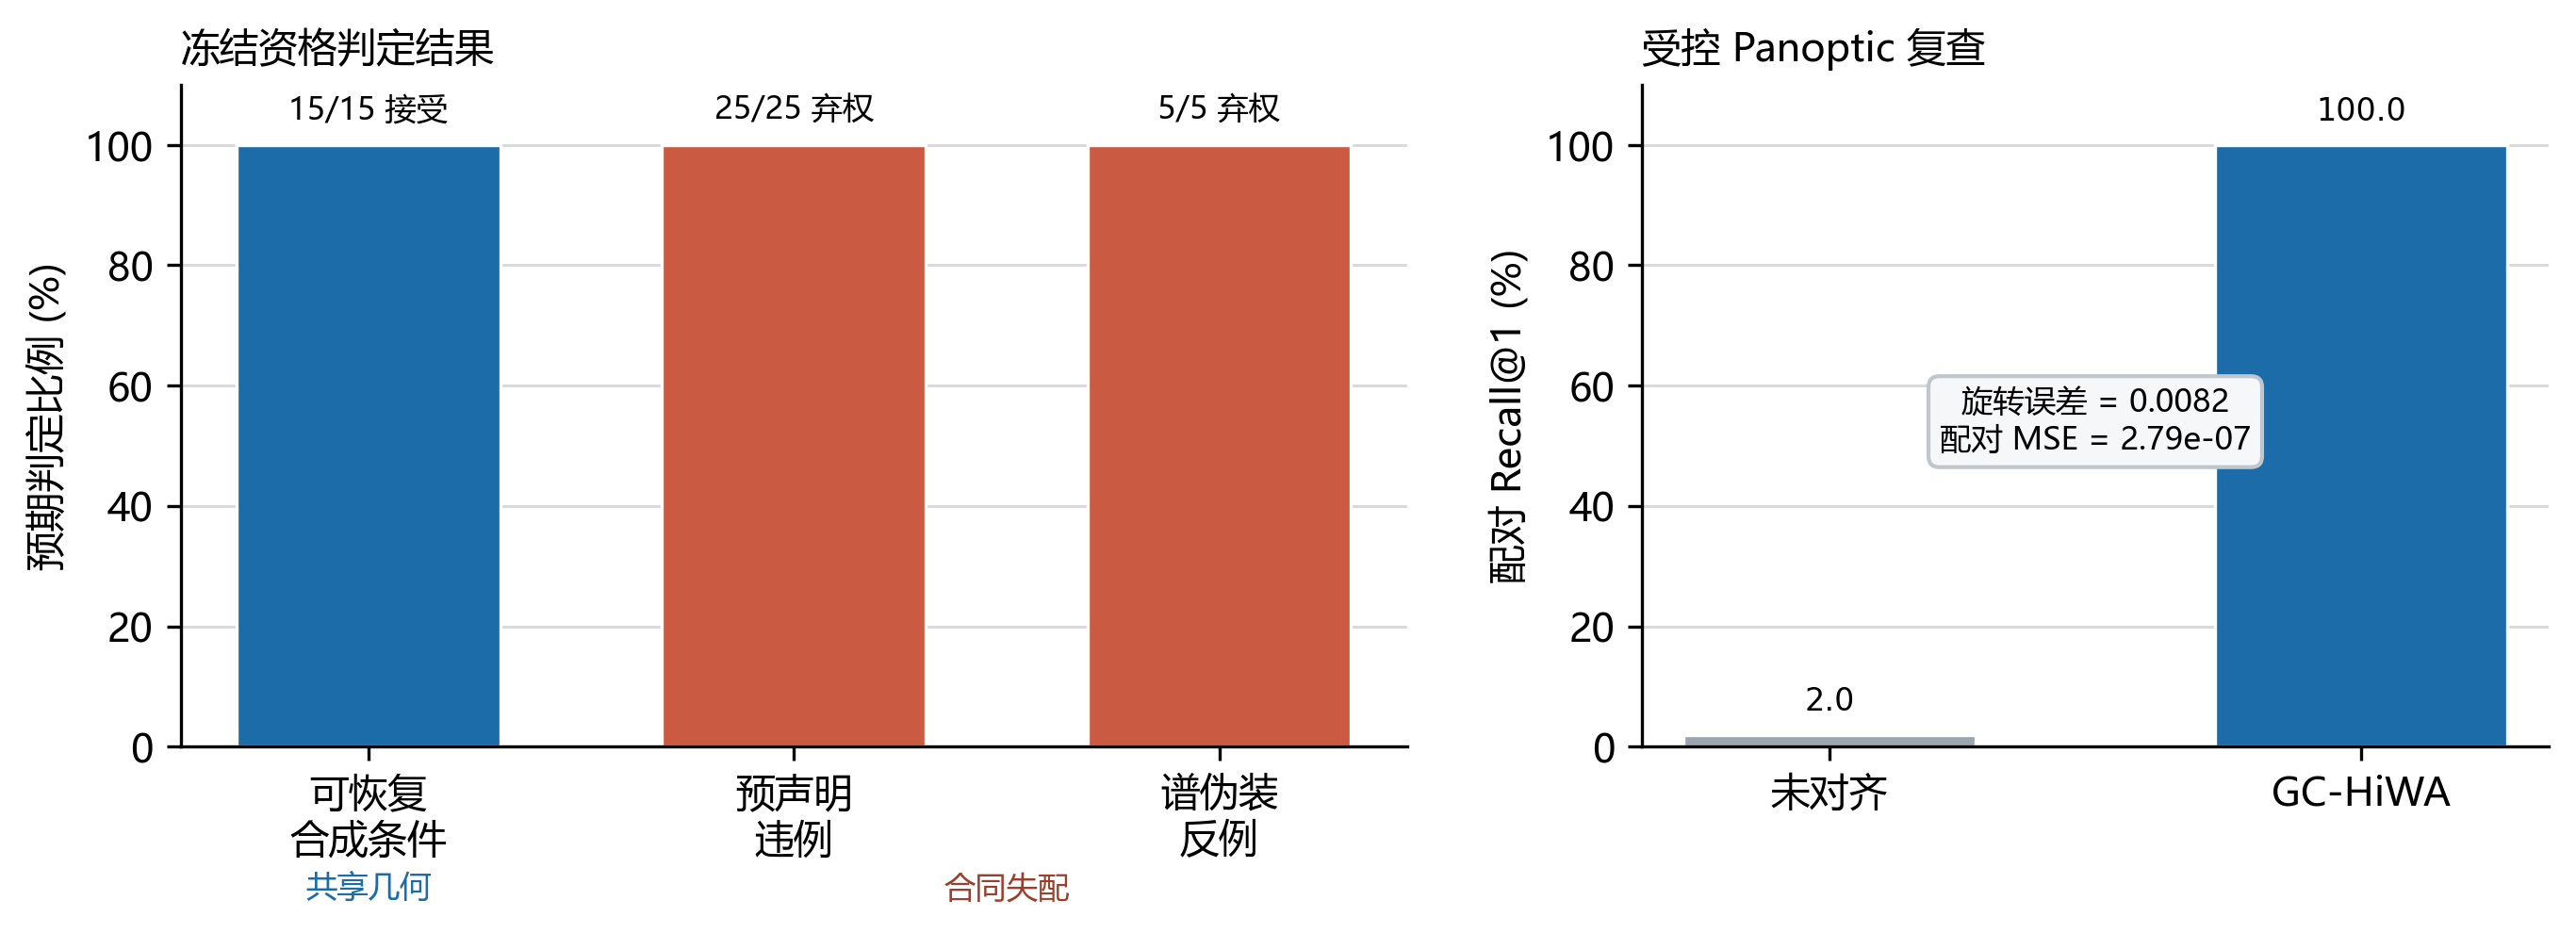
\includegraphics[width=\linewidth]{gc_hiwa_evidence_summary_cn.png}
\caption{冻结主证据汇总。左图报告三个独立合成条件下的预期资格判定：可恢复条件被接受，已声明违例和谱伪装反例均被弃权。右图为受控 Panoptic 跨相机复查的事后配对检索，未对齐基线为 $1.98\%$，通过 GC-HiWA 后为 $100\%$；框内给出相同冻结运行的旋转误差和配对 MSE。}
\label{fig:evidence-summary-cn}
\end{figure}

图 \ref{fig:evidence-summary-cn} 将三个合成判定与 Panoptic 受控复查放在同一证据视图中。左图中的颜色不是性能优劣，而是合同成立时的接受与合同被明确破坏时的弃权；右图则只衡量已知配对的坐标一致性，不应解释为跨相机的语义动作识别。该区分使“可恢复”与“应当不作映射声明”具有同等清晰的实验地位。

\subsection{Panoptic 中结构约束的必要性}
\begin{table}[H]
\centering
\caption{Panoptic Studio 的受控跨相机坐标恢复。}
\label{tab:panoptic}
\begin{tabularx}{0.96\linewidth}{lCCC Y}
\toprule
设置 & 有效运行 & 旋转误差 & Recall@1 & 结论\\
\midrule
无结构 $O(57)$ & 0/1 & 10.31 & -- & 100 轮未收敛，不能解释为相机变换\\
pose1，00\_00$\to$00\_01 & 5/5 & 均值 0.0154；最大 0.0254 & 1.0 & 结构化恢复\\
pose1，00\_00$\to$00\_05 & 3/3 & 最大 0.0308 & 1.0 & 不依赖单一相机对\\
pose1，00\_00$\to$00\_21 & 3/3 & 最大 0.0288 & 1.0 & 不依赖单一相机对\\
最终资格复查（seed 1601） & 1/1 & 0.00818 & 1.0 & paired MSE $2.79\times10^{-7}$，$\kappa_{\mathrm{id}}=0.133$\\
\bottomrule
\end{tabularx}
\end{table}

\subsection{MiHiA 开发比较、软聚合 HiWA 与 ROCA}
这一部分交代 GC-HiWA 的方法来处，而不是用 MiHiA 神经--运动开发结果替代当前的坐标恢复主证据。该开发比较使用一个固定、等距抽取的 $96\times96$ 源--目标子集：神经样本作为无标签对齐输入；运动方向标签和连续运动速度不进入原型学习、传输、旋转估计或分支选择，只在这些步骤完成后用于计算方向准确率和速度预测的决定系数 $R^2$。软聚合 HiWA 在 HiWA 的 Birkhoff 群组传输 $P$、每个群组对的局部 $Q_{ij}$ 与 $R_{ij}$、以及将局部变换压回一个全局 $R$ 的 ADMM 共识\cite{lee2019hierarchical} 上，加入可学习软原型、row-wise assignments 与列归一化的加权经验测度。在 full-support 设置中，每个 $Q_{ij}$ 都使用全部样本，唯一区别是 \cref{eq:local-marginals} 的软质量；而 $P$ 仍保持均匀群组边际。将 $P$ 错写成由软群质量决定的非均匀边际，会改变该基线的定义。

项目还测试过一个组件条件局部代价：对样本 $x_i,y_j$，以 $s_{ij}=a_i^X P(a_j^Y)^\top$ 表示其群组兼容性，并加入 $-\beta\log(s_{ij}+10^{-12})$。该项让上层群组关系影响下层样本运输。当前神经--运动 smoke 结果显示，能改变连续 $R^2$ 的 $\beta$ 会降低方向准确率，极小 $\beta$ 又没有稳定收益。因此最终主线令 $\beta=0$，把该项保留为负向机制证据，而非性能来源。

在 MiHiA 的 10 次运行（seeds 80--89）中，Hard HiWA、软聚合 HiWA 和软聚合 HiWA+ROCA 的平均方向准确率分别为 $0.4188,0.4271,0.4792$，运动 $R^2$ 分别为 $0.1908,0.1947,0.3364$；ROCA 在 10 次运行中事后选到较高准确率分支 8 次。此处标签只在分支确定后的最终指标中出现。故这些数值说明的是：在这一受限的神经--运动开发比较中，软测度与无标签分支资格值得继续审计；它们不构成 GC-HiWA 已在真实跨设备语义任务上优于所有方法的主张。

\begin{figure}[H]
\centering
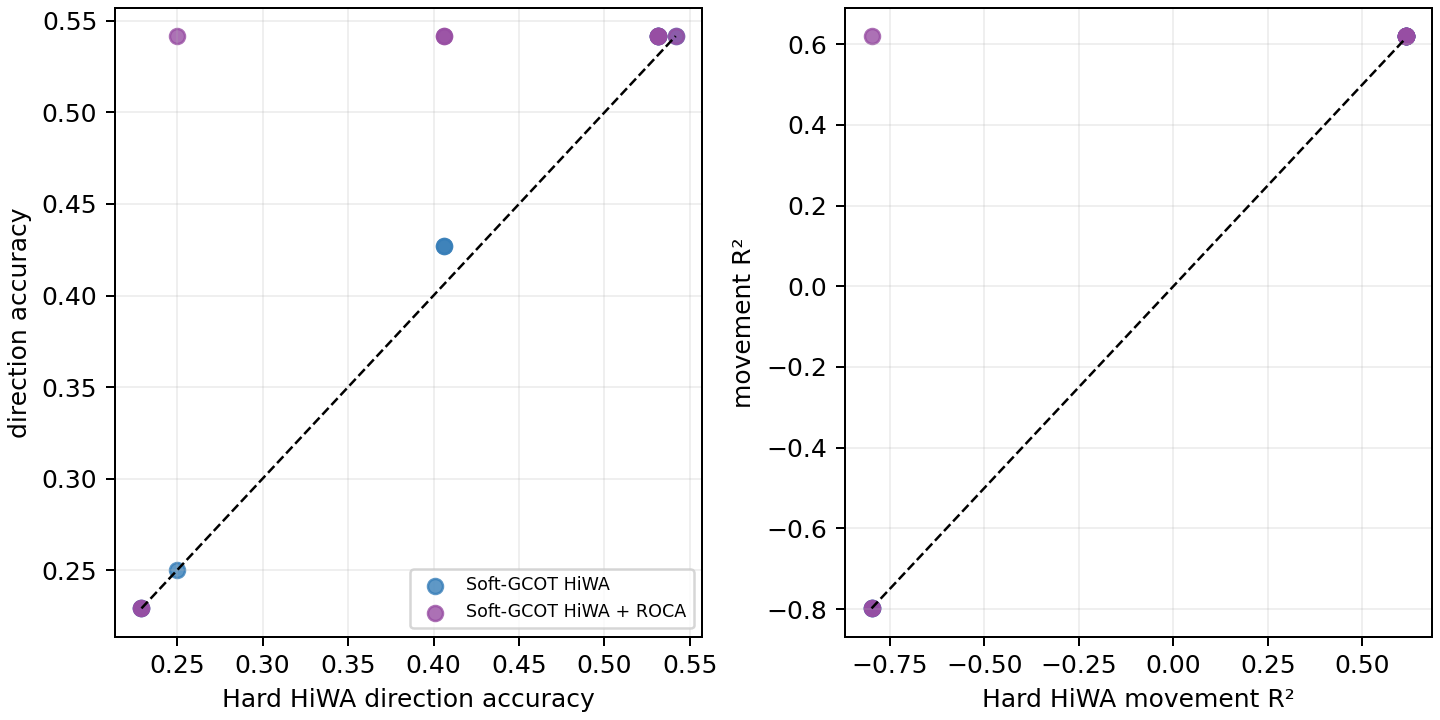
\includegraphics[width=0.86\linewidth]{paired_analysis_full_support_roca_seeds_80_89.png}
\caption{MiHiA $96\times96$ 神经--运动开发比较的配对分析（10 次运行）。它是软聚合 HiWA/ROCA 的机制证据，不是独立的 GC-HiWA 主验证，也不表示 ROCA 是无误选择器。}
\label{fig:roca-development}
\end{figure}

为避免单次好结果，进一步固定完整 pose2 序列并做多启动。主体 0、帧 141--339 的
00\_00 $\to$ 00\_01 设置中，5 次启动有 4 次形成 $5^\circ$ 内稳定簇，代表解误差为
0.00575、Recall@1 为 1；一个误差 0.716 的局部解与稳定簇相差约 $6.7^\circ$，因此被重启规则排除。
主体 2、帧 10000--10099 的独立窗口中，3/3 解在 $0.61^\circ$ 内一致，代表误差为
0.0435、Recall@1 为 1。

\subsection{冻结下游代理}
\begin{table}[H]
\centering
\caption{冻结源端姿态状态分类器的受控迁移代理。数值为普通准确率 / 平衡准确率。}
\label{tab:proxy}
\begin{tabular}{lccc}
\toprule
独立窗口 & 源域留出 & 目标原坐标 & 目标经 GC-HiWA\\
\midrule
主体 0，帧 141--339 & 0.888 / 0.864 & 0.838 / 0.333 & 0.888 / 0.864\\
主体 2，帧 10000--10099 & 0.600 / 0.822 & 0.250 / 0.667 & 0.575 / 0.811\\
\bottomrule
\end{tabular}
\end{table}

该表说明恢复后的坐标可使冻结源模型接近源域表现；第二窗口的普通准确率从 0.250 提升至 0.575。由于状态由源姿态自动定义，不能将这一结果升级为真实动作识别迁移。

\subsection{外部数据的负结果为何重要}
\begin{table}[H]
\centering
\caption{外部数据审计的结论。}
\label{tab:negative}
\begin{tabularx}{0.96\linewidth}{lYY}
\toprule
数据或方向 & 已执行的检查 & 不能作为主结果的原因\\
\midrule
Indy-Loco & 跨会话软聚合 HiWA、任务感知 OT、配对 Procrustes 上界 & 即使 oracle 上界也缺少有用转移，神经到瞬时速度不满足共同正交几何\\
PBMC RNA--ATAC & 共享特征、硬/软对齐、paired recall & 共享特征空间不等于可由正交变换恢复的共同几何\\
PAMAP2 & 时间安全协议、弱配对、多主体可用性 & 本地数据不足以支持跨主体结论，task-aware OT 无稳定收益\\
Paderborn & 工况/实体切分审计 & 一种切分饱和、另一种无信号，任务无法有效验证方法\\
\bottomrule
\end{tabularx}
\end{table}

\subsection{为何不将扩展模块写入主贡献}
我们比较了固定主干与联合原型更新；在种子 110--112 的已有机制检查中，平均方向准确率均为 0.5035，而联合版的速度 $R^2$ 从约 0.61996 微降至 0.61921。残差表示编码器的独立复核中，固定主干方向准确率为 0.4375，学习表示后为 0.1979，低于未对齐的 0.2708。它们不是“永远无效”，但没有显示稳定、独立、可复核的增益。

自动群组数也未满足准入标准。独立种子 2104--2108 的五群组合成检查中，固定 $K=4$ 为 5/5 接受且平均旋转误差 0.0109；事后知道真群数的 oracle $K=5$ 为 4/5 接受且平均误差 0.5429，并出现错误局部解。因此，截断 DP 或 DP-GMM 的复杂度目前没有实证回报。

\section{讨论}
\label{sec:discussion}

\subsection{当前可以得出的结论}
当前证据支持如下有限结论：当数据满足共享群组几何和预声明的结构化单旋转合同，GC-HiWA 能在无配对、无目标标签、无相机标定条件下恢复三维姿态坐标关系；当本文设计的失配出现时，组合资格检查倾向于弃权。合成结果说明恢复--弃权边界，Panoptic 结果提供受控真实几何证据。

\subsection{当前不能得出的结论}
\begin{quote}\small
\textbf{不可越过的解释边界。}
\begin{itemize}
  \item 本文不证明完整非凸 OT--ADMM 的全局收敛。
  \item 当前阈值不是未知分布上的错误接受率或错误弃权率保证。
  \item Panoptic 属于同一采集系统下的受控相机几何，不等于独立设备上的语义泛化。
  \item 冻结姿态状态代理不等于人工动作标签的跨设备动作识别。
  \item ROCA 不保证在任意数据集上选对分支；它在资格不足时应弃权。
\end{itemize}
\end{quote}

\subsection{真实语义验证的下一步}
UWA3D Multiview Activity II 提供 30 类动作、10 名受试者和四个 Kinect 视角，且各视角并非同步拍摄\cite{uwa3dii}。因此它适合测试“源视角有标签、目标视角无标签”的语义迁移，但不应报告不存在的帧级真旋转或帧配对。冻结协议应为：按受试者划分；在源视角训练动作分类器；仅用训练受试者的无标签目标视角拟合 GC-HiWA；在未见受试者目标视角上一次性打开标签评分；同时报告 source-only、未对齐、GC-HiWA、可用的标定式上界、接受率与弃权率。

\section{数据来源、使用方式与证据边界}
\textbf{合成数据}由三维群组点集生成：其一满足预先声明的单旋转合同，其余为预先声明的违例；它们只用于检验恢复与弃权。\textbf{Panoptic Studio 数据}为同一采集系统下相机对的 19 关节三维骨架；拟合时屏蔽相机外参、同步帧身份与标签，仅在事后打开这些信息进行坐标恢复评分。\textbf{MiHiA 神经--运动数据}用于上文的 $96\times96$ 开发比较；其中方向和速度结果仅用于最终评价。\textbf{Indy-Loco、PBMC RNA--ATAC、PAMAP2 与 Paderborn}只作为适用性边界的数据线：本文报告其结果是为了说明它们为何不能构成正向迁移主张。本文没有任何结果证明语义动作识别或普适的跨设备泛化。

\section{可复现性声明}
\label{sec:reproducibility}
核心实现位于 \url{src/cc_hiwa/}；合成边界运行器为 \url{experiments/synthetic/run_gc_hiwa_boundary_benchmark.py}；Panoptic 运行器位于 \url{experiments/panoptic/}。资格与 ROCA 的实现分别为 \url{src/cc_hiwa/alignment_qualification.py} 与 \url{src/cc_hiwa/roca_qualification.py}；冻结结果存放于 \url{experiments/results/}。

脚本 \path{experiments/synthetic/verify_gc_hiwa_v2_evidence.py} 机器核验本文的关键冻结数字：15/15 恢复、25/25 弃权、谱伪装反例 5/5 弃权，以及 Panoptic 的结构化资格、旋转误差、paired MSE 和 Recall@1。最近完整回归测试为 114 项通过。Windows 环境中以 \texttt{OMP\_NUM\_THREADS=1} 与 \texttt{MKL\_NUM\_THREADS=1} 运行测试，以规避偶发运行时多线程中止；这不改变模型超参数。

\section{结论}
GC-HiWA 将无监督坐标对齐表述为带适用性合同的恢复问题。其固定主干结合软群组、分层熵正则 OT、局部--全局结构化旋转共识与 ROCA 候选资格选择。合成边界、谱伪装反例和 Panoptic 受控实验共同支持一个谨慎主张：在共享几何与单一物理坐标变换存在时，方法可以恢复；在该合同冲突时，方法可以拒绝。下一阶段的关键不是叠加未经验证的编码器或自动聚类，而是在冻结协议下完成独立真实语义动作数据的验证。

\appendix
\section{符号表}
\begin{longtable}{p{0.29\linewidth}p{0.63\linewidth}}
\toprule
符号 & 含义\\
\midrule
\endfirsthead
\toprule
符号 & 含义\\
\midrule
\endhead
$X,Y$ & 源域与目标域无配对样本矩阵\\
$n,m,d$ & 源样本数、目标样本数与共同特征维数\\
$R_\star$ & 隐藏真坐标变换，仅用于合成或标定式评价\\
$\mathcal R$ & 预先声明的允许变换族\\
$I_J\otimes SO(3)$ & 所有关节共享一个三维旋转的姿态变换族\\
$a_{ik}^X,a_{j\ell}^Y$ & 样本对原型的软隶属度\\
$Z_X,Z_Y;\ C^X,C^Y;\ c_k^X,c_\ell^Y$ & 全局中心化、标量标准化后的样本；原型矩阵；及其原型行\\
$A^X,A^Y;\ K_X,K_Y;\tau_X,\tau_Y$ & 软隶属度矩阵；群组数；及软隶属度温度\\
$\alpha^{(k)},\beta^{(\ell)}$ & 第 $k,\ell$ 个局部 OT 的归一化边际\\
$Q_{k\ell}$ & 群组对 $(k,\ell)$ 的局部样本传输计划\\
$P,\mathcal V$ & 组间传输计划及其均匀边际可行集合\\
$R_{k\ell},R_g;\Pi_{\mathcal R};\Lambda_{k\ell}$ & 局部旋转、全局共识旋转、到允许族的投影及缩放 ADMM 对偶变量\\
$I_J;SO(3);O(d)$ & 关节块数为 $J$ 的单位矩阵、三维正旋转群及 $d$ 维全正交群\\
$D^{(k\ell)},C_{k\ell};\rho;w_{k\ell}$ & 局部平方距离代价、群组对代价、ADMM 惩罚系数及运输权重\\
$s_{ij};\beta;\lambda_H,\lambda_2$ & 组件相容性、其探索权重、及原型熵/尺度权重\\
$\varepsilon_{\mathrm{in}},\varepsilon_{\mathrm{out}}$ & 内层与外层熵正则强度\\
$\eta$ & 单旋转跨域拟合比\\
$\delta_{\mathrm{spec}}$ & 归一化协方差谱差\\
$\kappa_{\mathrm{id}}$ & 二阶几何可识别性间隔\\
$\pi,\widehat\pi$ & 潜在群组置换及由群组传输诱导的估计置换\\
$P_\pi;E_{k,r}(\delta);\delta$ & 置换计划、有限样本群组代价误差上界及其概率水平\\
$\varepsilon;X_{\mathrm{agg}},Y_{\mathrm{agg}};X_{\mathrm{agg}}^\dagger;C_X$ & Gram 扰动量、加权聚合矩阵、Moore--Penrose 伪逆及稳定性界常数\\
\bottomrule
\end{longtable}

\bibliographystyle{plain}
\begingroup
\small
\setlength{\parskip}{0pt}
\bibliography{references}
\endgroup

\end{document}
